\section{Red a analizar: estadísticos y análisis básico}

De cara a realizar esta práctica se va a analizar la red de seguidores de la Escuela Técnica Superior de Ingenierías Informática y de Telecomunicación (ETSIIT), de la Universidad de Granada.

He escogido esta red ya que me parece interesante estudiar las conexiones que puede tener la ETSIIT al ser un centro donde coinciden distintos perfiles, investigadores, estudiantes, docentes, empresas, instituciones, etc, lo que puede ser interesante ver y comprender como interactúan todo este tipo de perfiles, y observar si es fácil hacer estas distinciones entre perfiles.

\subsection{Obtención de los datos de la red}

Para obtener los datos de los seguidores de Twitter he utilizado la herramienta twitter-graph \cite{twitterGraph}. Esta herramienta permite utilizar nuestras credenciales de desarrollador de Twitter para realizar peticiones a la API de Twitter, como obtener los seguidores y conexiones de cierto usuario, buscar por términos concretos en todo Twitter, o obtener los me gusta a los que le ha dado un usuario.

En nuestro caso se ha utilizado para obtener los datos de los seguidores de la cuenta de la ETSIIT \cite{twitterETSIIT}. Al utilizar esta herramienta se nos ha generado dos ficheros csv, uno con los datos de los nodos y otro con la información de los enlaces.

\subsection{Previsualización de toda la red}

Una vez exportamos los datos a Gephi, podemos visualizar la red. De cara a poder visualizarla sin perder resolución, se ha exportado como PDF y se ha incrustado la página obtenida en esta memoria. Se ha utilizado el algoritmo ForceAtlas 2 para visualización, intentando que la red quede lo más estética posible, pero como vamos a ver se trata de una red muy densa, donde existen muchas conexiones y no es sencillo hacer un primer análisis visual claro.

Esta visualización es la generada directamente por Gephi, por lo que podemos hacer zoom a dicha visualización para poder ver en detalle la red.

\newpage
\begin{figure}[H]
	\centering
	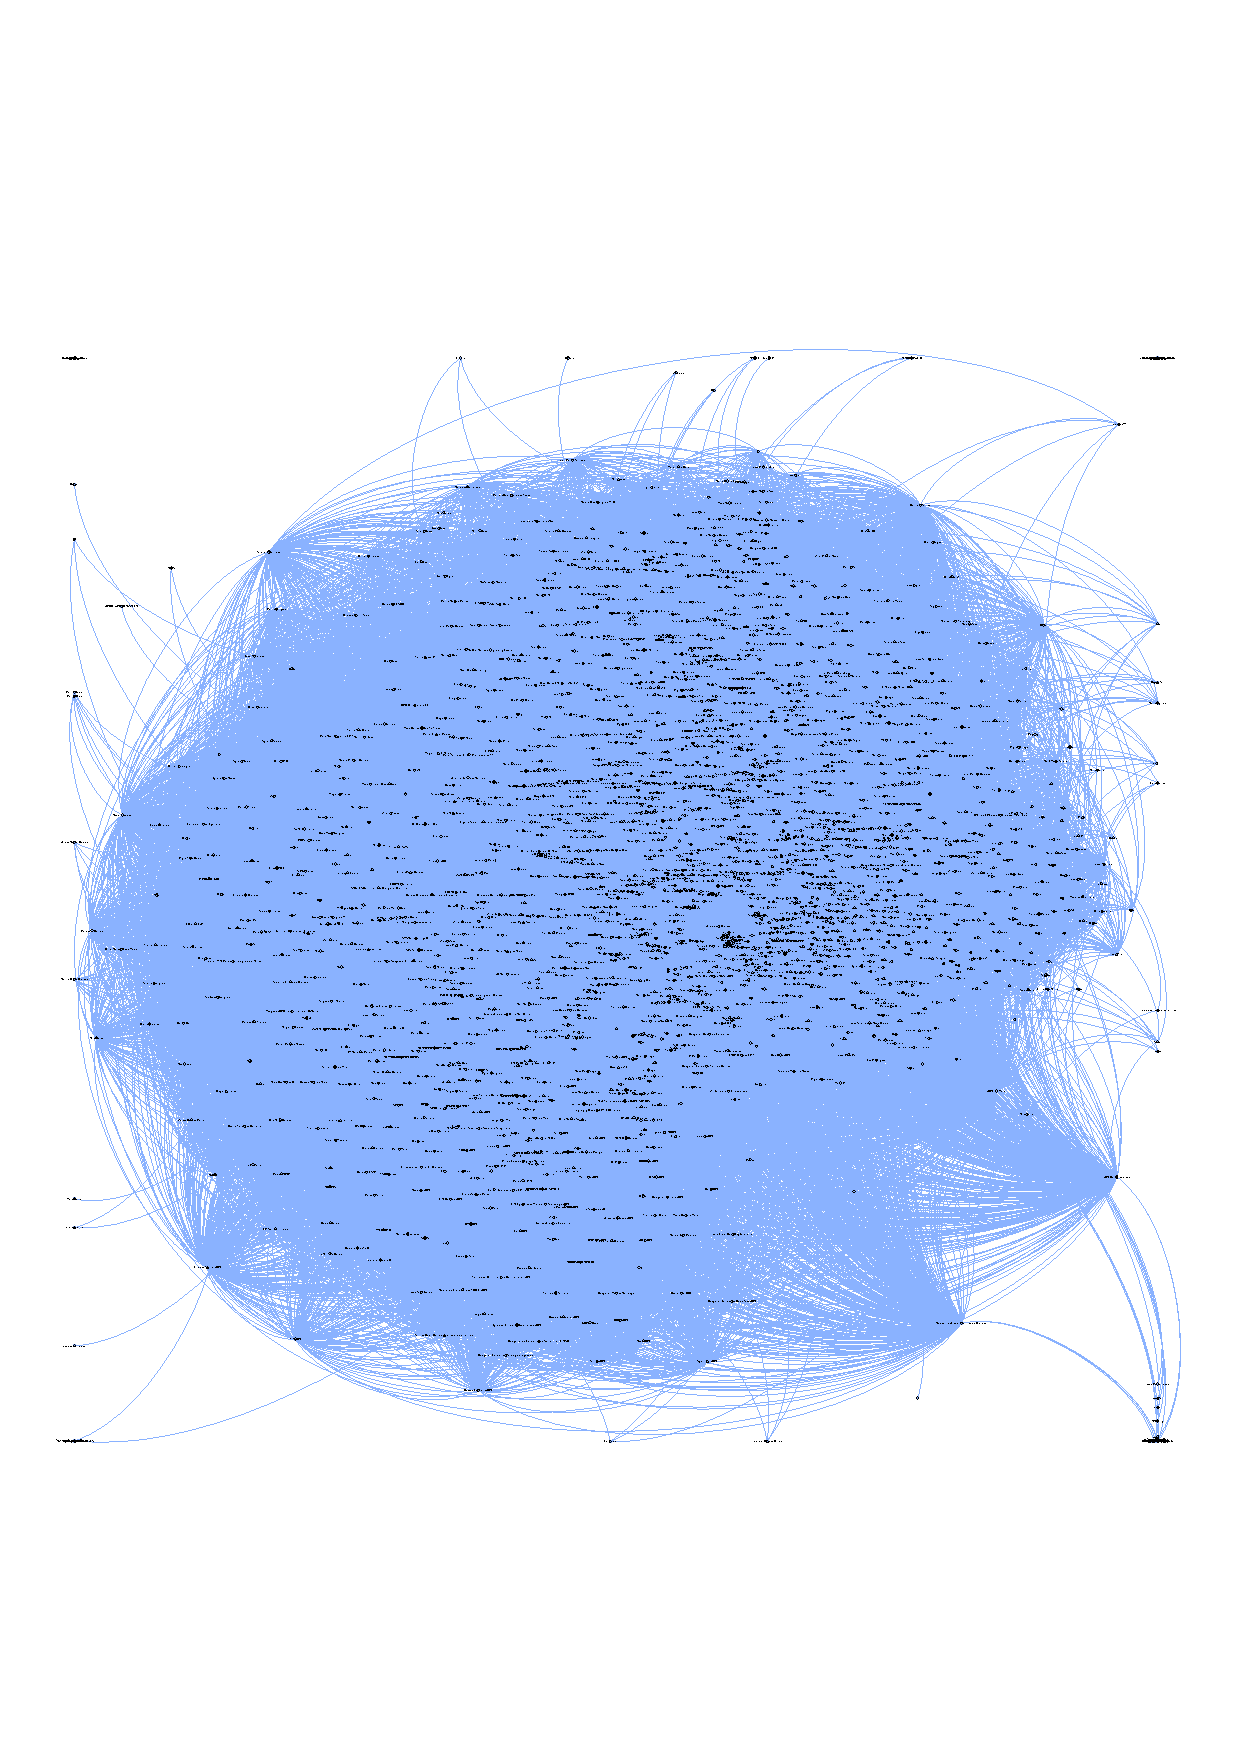
\includepdf[frame=true, scale=0.9, offset=75 -50]{pdf_incrustados/red_completa.pdf}
	\caption{Red completa de seguidores de la cuenta ETSIIT}
\end{figure}
\newpage


\subsection{Previsualización de la componente gigante de la red}

Con Gephi podemos observar el número de componentes conexos de la red, que en este caso son 65. Como podemos ver en el informe generado por Gephi, 64 de estas son nodos sin conexiones y la componente gigante contiene la mayor parte de los nodos y todas las conexiones:


\begin{figure}[H]
  \centering
  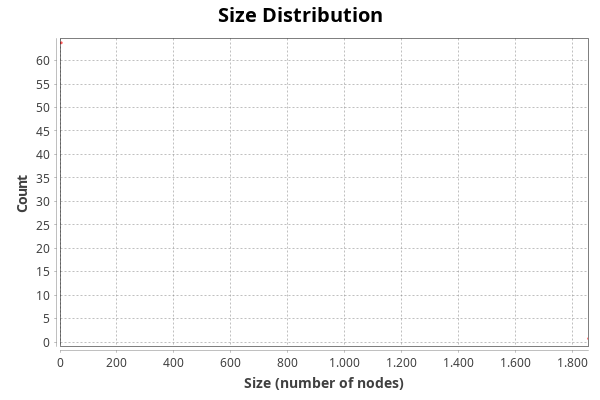
\includegraphics[width = \textwidth]{componentes_conexos.png}
  \caption{Informe sobre componentes conexos de Gephi sobre la red de seguidores de la ETSIIT.}
  \label{fig:componentes_conexos}
\end{figure}

Vamos a visualizar la red únicamente con la componente gigante, que como veremos, no aparecerán los nodos en los extremos que podíamos ver en la red completa.

\newpage
\begin{figure}[H]
	\centering
	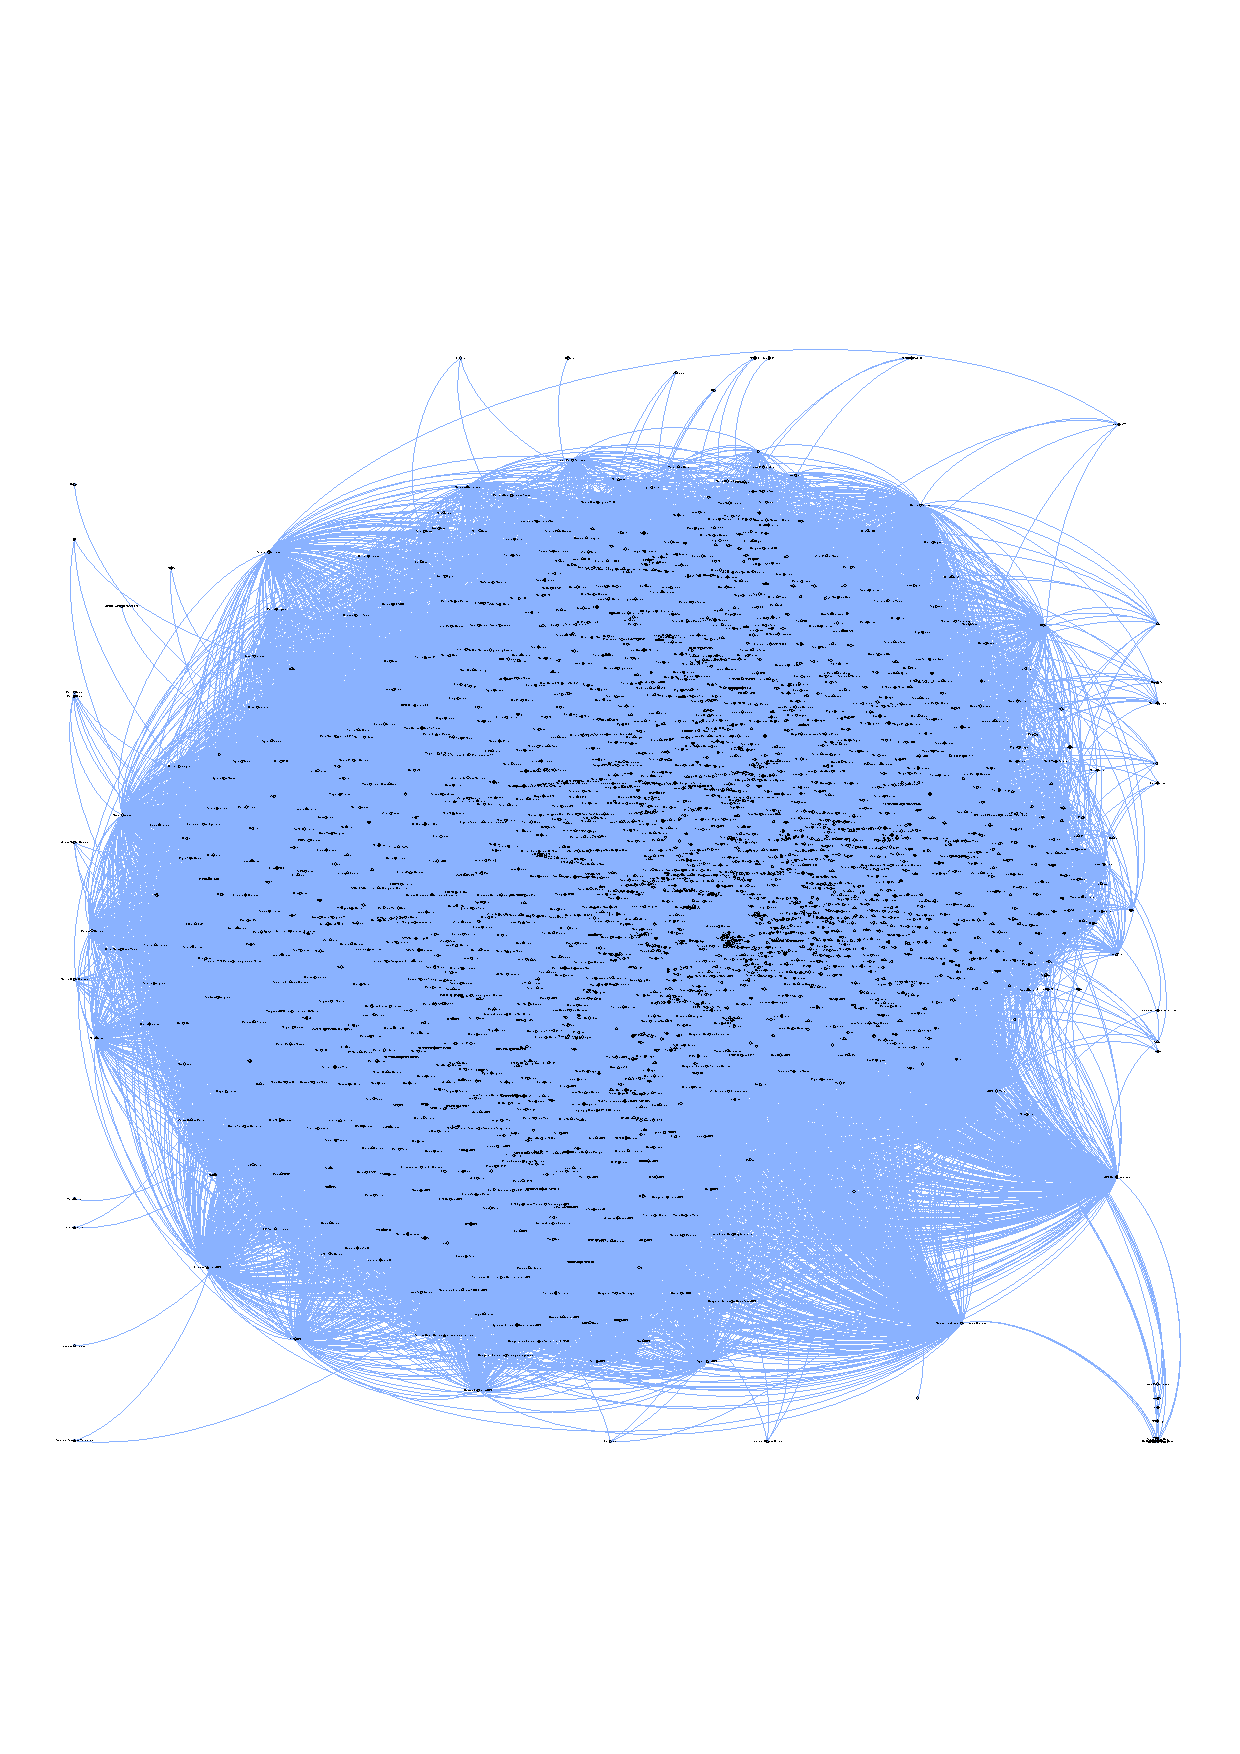
\includepdf[frame=true, scale=0.9, offset=75 -50]{pdf_incrustados/componente_gigante.pdf}
	\caption{Componente gigante de seguidores de la cuenta ETSIIT}
\end{figure}
\newpage

\subsection{Medidas de la red}

Como se pedía en el guión de prácticas, también se ha obtenido diversas medidas estadísticas sobre la red:

% Please add the following required packages to your document preamble:
% \usepackage{graphicx}
\begin{table}[H]
\centering
\begin{tabular}{|l|r|}
\hline
\multicolumn{1}{|c|}{\textbf{Medida}}                      & \multicolumn{1}{c|}{\textbf{Valor}} \\ \hline
Número de nodos N                                          & 1916                                \\ \hline
Número de enlaces L                                        & 47334                               \\ \hline
Número máximo de enlaces Lmax                              & 3.669.140                           \\ \hline
Densidad del grafo L/Lmax                                  & 0,013                               \\ \hline
Grado medio \textless{}k\textgreater{}                     & 24,705                              \\ \hline
Diámetro dmax                                              & 7                                   \\ \hline
Distancia media d                                          & 2,598965954                         \\ \hline
Coeficiente medio de clustering \textless{}C\textgreater{} & 0,407                               \\ \hline
Número de componentes conexas                              & 65                                  \\ \hline
Número de nodos componente gigante (y \%)                  & 1852 (0,966)                        \\ \hline
Número de aristas componente gigante (y \%)                & 47334 (1)                           \\ \hline
Diámetro dmax componente gigante                           & 7                                   \\ \hline
Distancia media d componente gigante                       & 2,598965954                         \\ \hline
\end{tabular}%
\caption{Medidas estadísticas de la red de seguidores de la ETSIIT}
\end{table}

Con estos datos podemos observar que tenemos una red con bastantes nodos pero muy poco densa globalmente (tenemos una densidad de grafo muy baja), también podemos ver que se trata de una red bastante conexa, en la que el diametro máximo es 7 y la distancia media es muy baja, ya que no llega a tres nodos.

Aunque la densidad de la red es baja, con el coeficiente medio de clustering podemos ver que la densidad local es bastante alta, es decir, hay una alta proporción de vecinos de cada nodo conectados.

Con respecto al número de componentes conexas, ya hemos visto en figuras anteriores como tenemos bastantes nodos sueltos y una componente gigante que abarca casi toda la red, cosa que confirmamos ahora al ver que todas las conexiones de la red están en la componente gigante de la red.

\subsection{Gráficos sobre las medidas de la red}

De cara a calcular las medidas de la sección anterior también se han obtenido diferentes gráficos sobre las medidas de la red.

Comenzando por los gráficos de distribución de grado, que al ser una red dirigida tenemos gráficos tanto de grado de entrada como grado de salida, así como el grado total:

\begin{figure}[H]
  \centering
  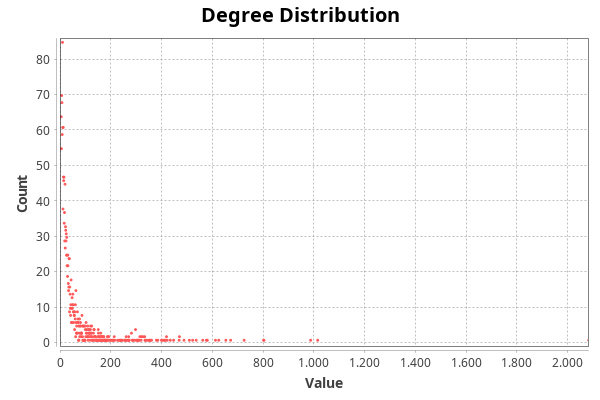
\includegraphics[scale = 0.5]{degree-distribution.png}
  \caption{Informe sobre la distribución de grados de la red de seguidores de la ETSIIT.}
  \label{fig:degree-distribution}
\end{figure}

\begin{figure}[H]
  \centering
  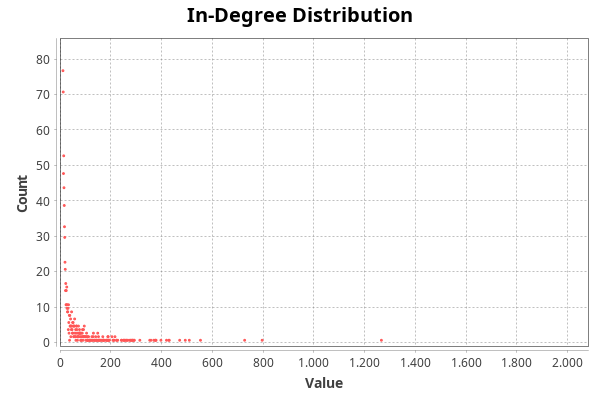
\includegraphics[scale = 0.5]{indegree-distribution.png}
  \caption{Informe sobre la distribución de grados de entrada de la red de seguidores de la ETSIIT.}
  \label{fig:indegree-distribution}
\end{figure}

\begin{figure}[H]
  \centering
  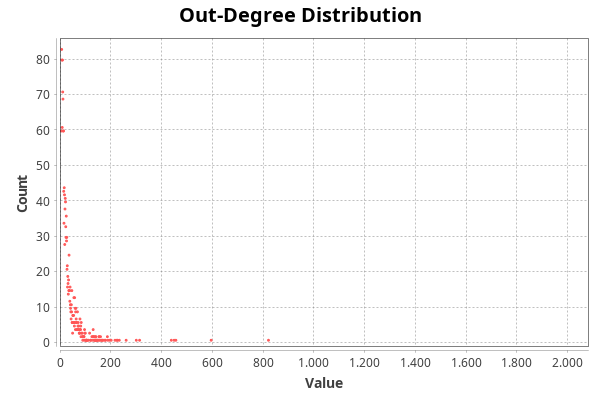
\includegraphics[scale = 0.5]{outdegree-distribution.png}
  \caption{Informe sobre la distribución de grados de salida de la red de seguidores de la ETSIIT.}
  \label{fig:outdegree-distribution}
\end{figure}

Con estos gráficos podemos ver que se trata de una red libre de escala, en la que la mayoría de los nodos apenas tienen enlaces, mientras que la mayoría de enlaces los tienen muy pocos nodos, llegando a tener un nodo con más de dos mil enlaces. Más adelante estudiaremos cuales son estos nodos con más conexiones y veremos si tienen sentido en la red sobre la que estamos trabajando.

También hemos obtenido (usando LibreOffice Calc ya que Gephi por error mostraba el gráfico vacío) la distribución del valor de coeficiente de clustering de los nodos:

\begin{figure}[H]
  \centering
  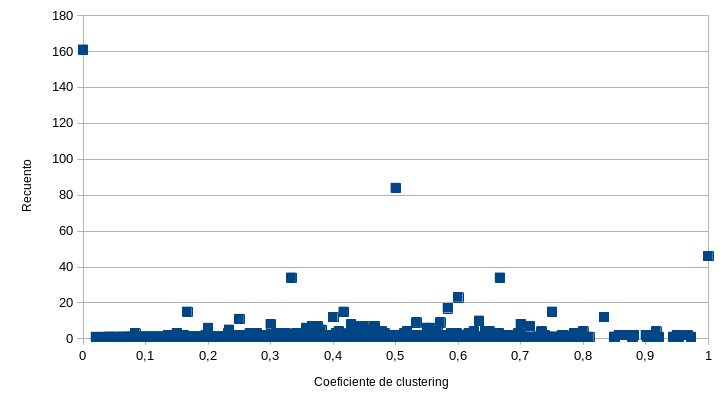
\includegraphics[scale = 0.6]{coeficiente_clustering.png}
  \caption{Informe sobre el coeficiente de clustering de los nodos de la red de seguidores de la ETSIIT.}
  \label{fig:outdegree-coeficiente_clustering}
\end{figure}

Vemos que hay muchos nodos (160 aproximadamente) con un coeficiente de clustering con valor 0, la densidad local de dichos nodos es nula, es decir, no tienen vecinos conectados. Por otro lado vemos que también destacan los valores 1 y 0.5, vemos como hay alrededor de 82 nodos con la mitad de sus vecinos conectados y encontramos unos 45 nodos en los que todos los vecinos están conectados. Estos valores nos dan a entender que la red es localmente densa, por lo que encontraremos hubs dentro de la red.
